% Personally, I prefer to use the aspectratio=169 option to set the aspect ratio of the slides to 16:9. 
% This is because most of the screens are in 16:9 aspect ratio nowadays. 
% If you prefer the 4:3 aspect ratio, you can remove this option.
\documentclass[aspectratio=169]{beamer}
\usetheme{MyCUHK}

\title{Your splashing title}

\author{Your Noble Name}

\institute{Your sweet CUHK}

\collaborators{Your bosses, students, and colleagues}
% If you don't need this entry, you can leave it empty, just like the following line.
% \collaborators{}

\occasion{Your grand occasion}
% If you don't need this entry, you can leave it empty, just like the following line.
% \occasion{}

\titlegraphic{

\includegraphics[height=1.0cm]{figs/cuhk-logo.png}
}
% Add more logos if you want to, but remember to adjust the height parameter accordingly.

\begin{document}
\begin{frame}[plain]
  \maketitle
\end{frame}

\section{Introduction}
\begin{frame}{What you can get from this template}
  \begin{itemize}
    \item Items in CUHK-purple.
    \item \alert{Alert text} in CUHK-brown.
    \item A separation line, sometimes you need it.
    \item A block to put your theorem, lemma, etc.
    \item You can put a border around a figure, see the next slide.
    \item A thanks page.
  \end{itemize}

  \MyCUHKline

  \begin{MyCUHKblock}{Riemann--<Your name> Theorem}
    The Riemann Hypothesis is \alert{true}.
  \end{MyCUHKblock}
\end{frame}

\begin{frame}{What you can get from this template}

  \begin{figure}
    \begin{MyCUHKfigure}
      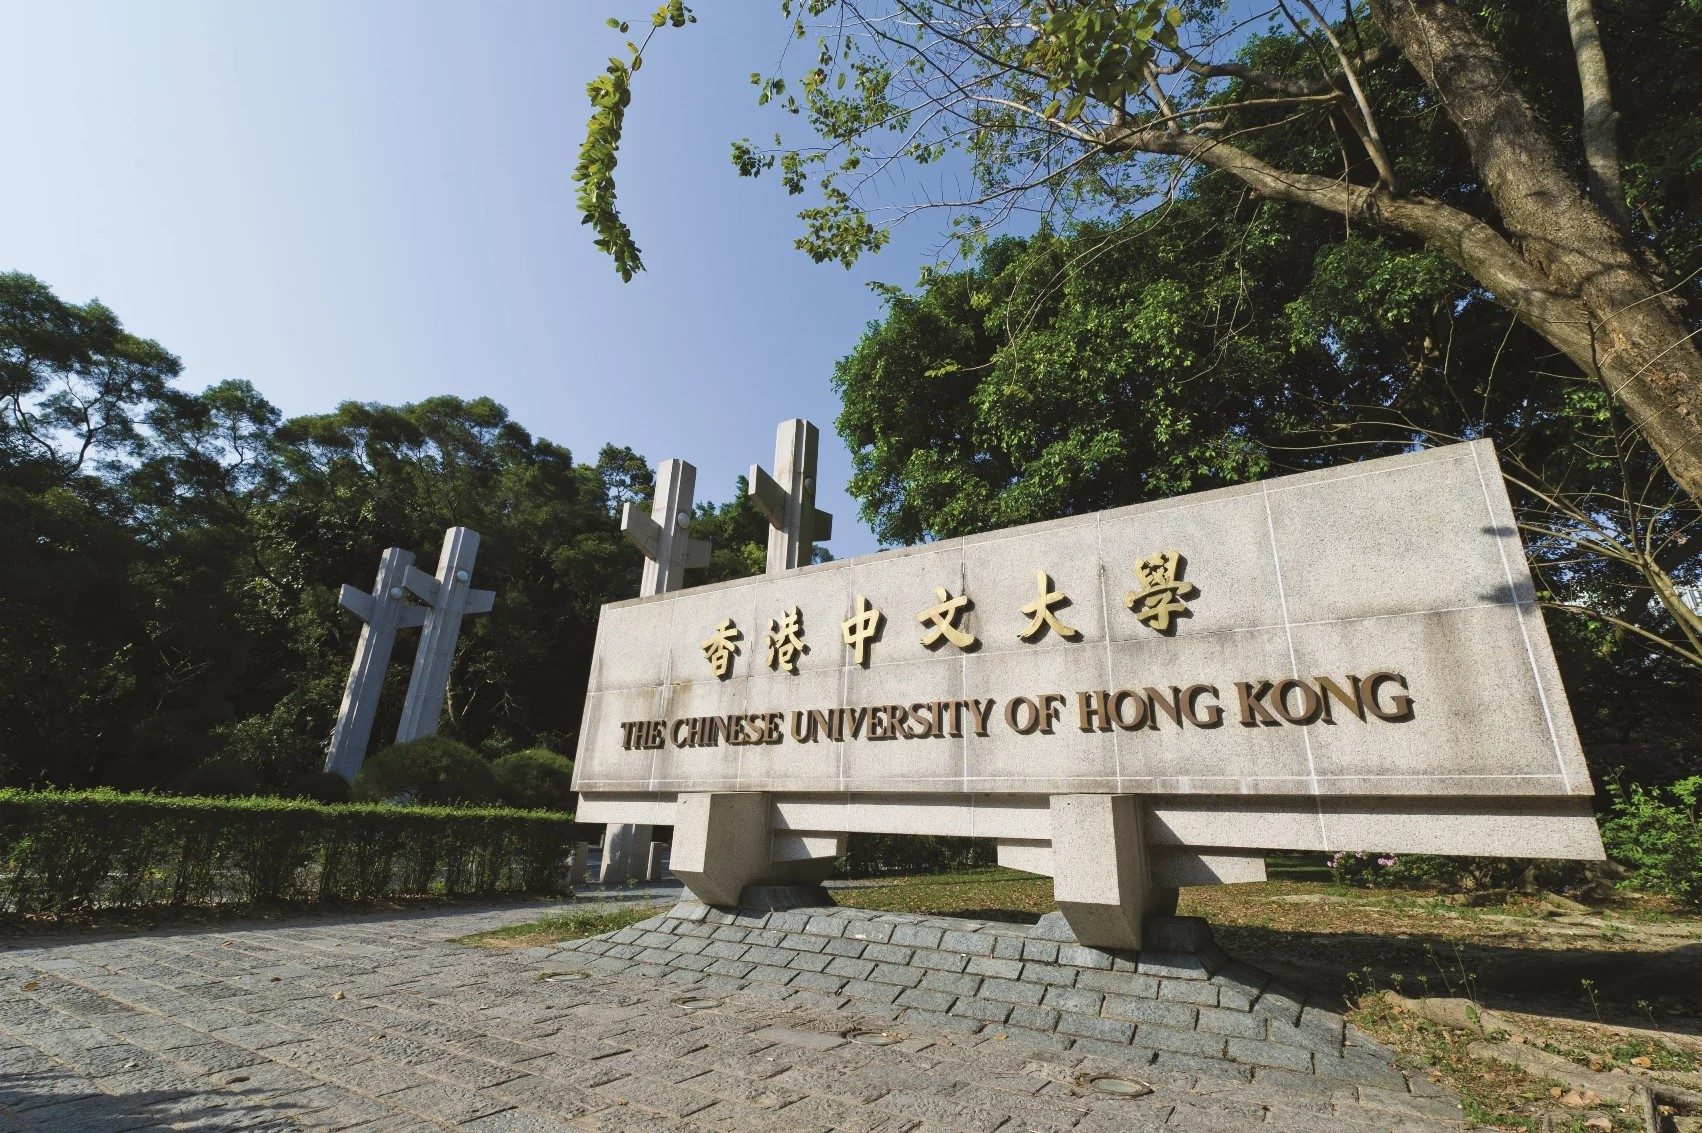
\includegraphics[width=0.3\textwidth]{figs/figure-from-web.jpeg}
    \end{MyCUHKfigure}
    \caption{A caption for the figure (just for demonstration).}
  \end{figure}

  You may notice that the background color is \alert{not} pure white.
  I provide a border around the figure to make a natural color transition.
\end{frame}

\begin{frame}{Before the ending}
  \begin{enumerate}
    \item This is a \alert{minimalist} template, you can add more features if you want.
    \item Do \alert{not} be afraid of those \LaTeX\ commands.
    \item Check the \alert{source code} to see how I \textcolor{CUHKyellow}{{\tiny copy}} implement those features.
    \item Use \alert{LuaLaTex} to unlock the full potential of Beamer!
  \end{enumerate}

\end{frame}

\thankspage{Thanks for your attention!}

\end{document}